\chapter{Related Works}

\section{Life-like CA}
\section{Reaction-diffusion CA}
\section{Learning CA with Evolutionary Algorithm}

\noindent
\textbf{Learning Algorithm for Modeling Complex Spatial Dynamics} (Meyer, Richards, and Packard, 1989) \cite{meyer1989learning} is a seminal work that uses genetic algorithms to learn cellular automata neighbourhood functions. It evolves a binary probabilistic cellular automaton (PCA) to model artificially generated datasets. The motivation is to establish a CA architecture to codify patterns in physical interactions directly from experimental data. In particular, Richards et al. \cite{richards1990extracting} uses PCA rules to predict the the dendritic solidification structure of NH\textsubscript{4}BR.\\

Note that the goal is not to learn the entire transition function of the cellular automaton. This work aims to establish \textit{which} parameters in a local vicinity of a current cell are most relevant to predicting the future state, not \textit{how} those parameters are combined and transformed to produce the result.\\

The search space is a 20-cell vicinity where each cell can be included or excluded from the neighbourhood set. It is the intersection of the Moore neighbourhood in time step $t-1$ and the von Neumann neighbourhood of range 2 in time step $t-2$ as visualised in Figure~\ref{fig:20-near}.

\begin{figure}[!h]
\centering
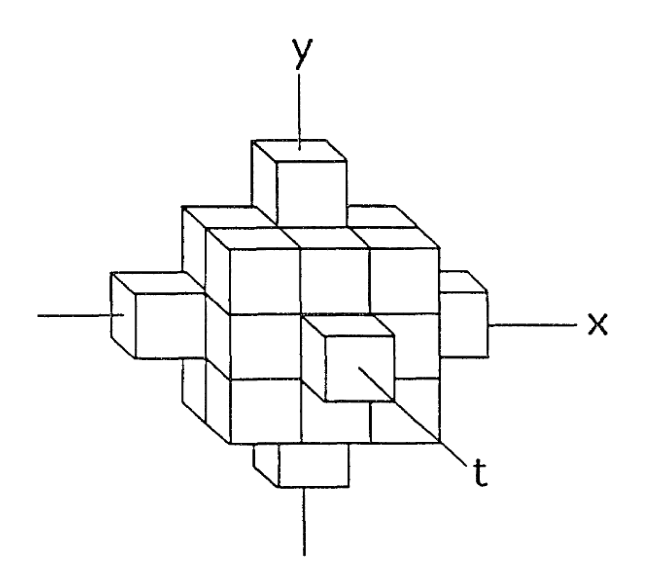
\includegraphics[width=0.3\textwidth]{images/20_neighbourhood.png}
\caption{20-cell, two step neighbourhood in space and time}
\label{fig:20-near}
\end{figure}

The full 20-cell neighbourhood is called the master template and each chromosome encodes some subtemplate ${s_1, ..., s_m}$. The fitness function used is
\begin{align*}
                    F &= I - \frac{2^m}{N}\\
    \text{where\:}  I &= \sum P(s, s_1, ..., s_m)\log_2{\frac{P(s, s_1, ..., s_m)}{P(s)P(s_1, ..., s_m)}}
\end{align*}
Here, $I$ is the mutual information of the subtemplate and represents the amount of information, measured in Shannon bits, that can be obtained about the value of the central cell from subtemplate states. It is calculated by summing across all $2^m$ configurations of the subtemplate in the data and across both values of $s \in \{0,1\}$. The second term in the fitness function ensures that subtemplates of varying sizes are treated appropriately by proportionately penalising large subtemplates that, by nature, will contain more information. $N=20$ is the size of the master template\\

The genetic algorithm initialises the population at a randomly chosen subset of possible subtemplates. Selection is performed using a truncated linear ranking. Crossover is applied using an arbitrary cut in space-time on the master template as the crossover point. Point mutation is applied by either adding or removing a single cell from each candidate. This process is iterated to converge towards an optimum.\\

This method precisely learns neighbourhoods interior to the master template such as the 1 time step Moore neighbourhood. Even when the objective neighbourhood lies partially outside the master template, the algorithm successfully finds a close approximation. For example, when given data produced by a 1 time step von Neumann neighbourhood, the algorithm learns a neighbourhood set that produces correct behaviour 96\% of the time.\\

As the first notable exploration of learning CA properties with genetic algorithms, this paper demonstrates the ability of GAs to efficiently traverse an opaque search space and approximate solutions to goals outside the search space.\\

This work also raises many questions for future research. The most pertinent is whether it is possible to link learned rules to existing and future theoretical models. Moreover, this work only explores binary state CA but application of similar techniques on continous-state CA could closer approximate the partial differential equations that underlie the physical processes being modelled.\\

Finally, this paper focuses on optimising the neighbourhood set of the CA model only. In this thesis, we are interested in going beyond this and approximating the full transition function. In some cases we will fix the neighbourhood function used to reduce our search space under the assumption that techniques from this paper can be used to find optimal sub-neighbourhoods if they exist.\\

\noindent
\textbf{Evolving Cellular Automata with Genetic Algorithms} (Mitchell, Crutchfield, and Das, 1996) \cite{mitchell1996evolving} shows the effectiveness of genetic algorithms in learning elementary cellular automata for global learning tasks such as the infamous density classification[CITE] and synchronisation[CITE] problems.\\

